\section{Droplet Curve in the Charge, Dielectric, and Slit Case}
\subsection{A Derivation from $w(\zeta)$}
We apply the complex potential from section (\ref{cpt:pot_zeta}) to calculate the thin film's height in the electric field of the charge embedded in the dielectric. it requires using the complex potential above $y=0$ to derive the height:
\[
w(\zeta) = \frac{q_t}{2\pi \epsilon_0} \im \left[ \log(\zeta - \zeta_0) - i \log\left(\frac{1}{\zeta} - \overline{\zeta_0}\right) \right]
\]
 define $\frac{q_t}{2\pi \epsilon_0}\im\coloneqq 1$ for convenience, therefore
\[
\frac{dw}{d\zeta} \sim  \frac{1}{\zeta - \zeta_0} - \frac{1}{\frac{1}{\zeta} - \overline{\zeta_0}} \cdot \frac{-1}{\zeta^2} =  \frac{1}{\zeta - \zeta_0} + \frac{1}{\zeta + \zeta^2\overline{\zeta_0}} 
\]
Apply $\zeta = e^{\im\theta}$ for the disc's upper curve on the $\zeta$-plane, and it will map to
\[
z = \frac{\zeta + \frac{1}{\zeta}}{2} = \cos \theta =x
\]
For the upper curve of the droplet, $\theta\in(0,\pi)$ and $x\in(1,-1)$, the surface charge density, $\sigma$, as a function of $\theta$, is
\[
\sigma(\theta) = \left| \frac{dw}{d\zeta} \frac{d\zeta}{dz} \right| (\theta)= \frac{q_t}{2\pi \epsilon_0}\left| \frac{1}{e^{i\theta} - \zeta_0} + \frac{1}{e^{i\theta} + e^{i2\theta}\overline{\cdot \zeta_0}} \right| \cdot \frac{1}{\sin \theta}
\]
We can rewrite $\sigma$ as  a function of $x$
\[
\sigma(x) = \frac{q_t}{2\pi \epsilon_0}\left| \frac{1}{x+\im\sqrt{1-x^2} - \zeta_0} + \frac{1}{x+\im\sqrt{1-x^2} + (x+\im\sqrt{1-x^2})^2\overline{\cdot \zeta_0}} \right| \cdot \frac{1}{\sqrt{1-x^2}}
\]
In this way, the surface charge density is derived from the complex potential on the $\zeta$-plane. However, the droplet's height from this equation would be complicated, so we attempt an alternative derivation starting from $w(z)$.

\subsection{Droplet's Height from $w(z)$}
The complex potential from above, on the $z$-plane, from section (\ref{cpt:slit_pot}) is\vspace{-.5em}
\[
w = i \underbrace{\log \left( z + \sqrt{z^2 - 1} - \zeta_0 \right)}_{w_1} - i \underbrace{\log \left( \frac{1}{z + \sqrt{z^2 - 1}} - \overline{\zeta_0} \right)}_{w_2}
\]
We work out $\sigma$ by $w_1$ and $w_2$.
\[
\frac{\partial w_1}{\partial z} = \frac{1}{z + \sqrt{z^2 - 1} - \zeta_0} \cdot \left( 1 + \frac{z}{\sqrt{z^2 - 1}} \right)= \frac{1}{\sqrt{z^2 - 1}} \cdot \frac{z + \sqrt{z^2 - 1}}{z + \sqrt{z^2 - 1} - \zeta_0}
\]
on the slit, we have \( z = x \), and \( x \in (0,1) \), let $\zeta_0\coloneqq-a\im$, then
\[
\frac{\partial w_1}{\partial z} \Bigg|_{z=x} = \frac{1}{\im\sqrt{1 - x^2}} \cdot \frac{x + i \sqrt{1 - x^2}}{x + i \left( a + \sqrt{1 - x^2} \right)}
\]
take the absolute value to obtain $\sigma_1$
\begin{equation*}
    \begin{split}
        \left| \frac{\partial w_1}{\partial z} \right|_{z=x}&= \frac{1}{\sqrt{1 - x^2}} \cdot \frac{\left|x + i \sqrt{1 - x^2}\right|}{\sqrt{x^2 + a^2 + \left( \sqrt{1 - x^2} \right)^2 + 2a \sqrt{1 - x^2}}}\\
        &= \frac{1}{\sqrt{1 - x^2}} \cdot \frac{1}{a^2 + 1 + 2a \sqrt{1 - x^2}}
    \end{split}
\end{equation*}
The absolute value sign is removed since:\vspace{-.5em}
\[
a^2 + 1 + 2a \sqrt{1 - x^2}>a^2 + 1 + 2a=(a+1)^2\geq 0\vspace{-.5em}
\]
Next, we derive the surface charge density of $w_2$ .
\begin{equation*}
    \begin{split}
    \frac{\partial w_2}{\partial z} &= -i \cdot \frac{1}{\frac{1}{z + \sqrt{z^2 - 1}} - \overline{\zeta_0}} \cdot \left(\frac{1}{z+\sqrt{z^2 - 1}}\right)'\\
    &= -i \cdot \frac{z + \sqrt{z^2 - 1}}{1 - \overline{\zeta_0}\left(z + \sqrt{z^2 - 1}\right)} \cdot \frac{-1}{\left(z+\sqrt{z^2 - 1}\right)^2} \cdot \left( 1 + \frac{z}{\sqrt{z^2 - 1}} \right)\\&= \frac{i}{\sqrt{z^2 - 1}} \cdot \frac{z + \sqrt{z^2 - 1}}{1 - a i \left( z + \sqrt{z^2 - 1} \right)}\\
    &= \frac{i}{\sqrt{z^2 - 1}} \cdot \frac{z + \sqrt{z^2 - 1}}{1 - a i \left( z + \sqrt{z^2 - 1} \right)}
    \end{split}
\end{equation*}

Similiar to the $w_1$ derivation, we have \( z = x \) on the slit, therefore\vspace{-0.5em}
\[
\frac{\partial w_2}{\partial z} \Bigg|_{z=x} = \frac{\im}{\im\sqrt{1 - x^2}} \cdot \frac{1}{1 - a i x - a \im\im \sqrt{1 - x^2}}\vspace{-0.5em}
\]
Take the absolute value to obtain $\sigma_2$ this time\vspace{-0.5em}
\begin{equation*}
    \left| \frac{\partial w_2}{\partial z} \right|_{z=x}= \frac{1}{\sqrt{1 - x^2}} \cdot \frac{1}{\sqrt{(1 + a \sqrt{1 - x^2})^2 + (a x)^2}}= \frac{1}{\sqrt{1 - x^2}} \cdot \frac{1}{1 + a^2 + 2 a \sqrt{1 - x^2}} \vspace{-0.5em}      
\end{equation*}
Therefore, the surface charge densities $\sigma_1$, and $\sigma_2$ of $w_1$, and $w_2$, are found to be equal. We sum the two to obtain the complete surface charge densities.\vspace{-0.5em}
\[
\left|\frac{\df w}{\df z}\right|_{z=x}=\left|\frac{\df w_1}{\df z}+\frac{\df w_2}{\df z}\right|_{z=x} = \frac{2}{\sqrt{1 - x^2}} \cdot \frac{1}{1 + a^2 + 2 a \sqrt{1 - x^2}}\vspace{-0.5em}
\]
We omitted some constants in the derivation, as we are working with the non-dimensional equation. Hence, for the surface charge density on the upper slit, $\sigma$, we find\vspace{-0.5em}
\[
\sigma\sim \frac{2}{\sqrt{1 - x^2}} \cdot \frac{1}{1 + a^2 + 2 a \sqrt{1 - x^2}}\vspace{-0.5em}
\]
\begin{figure}[H]
    \centering
    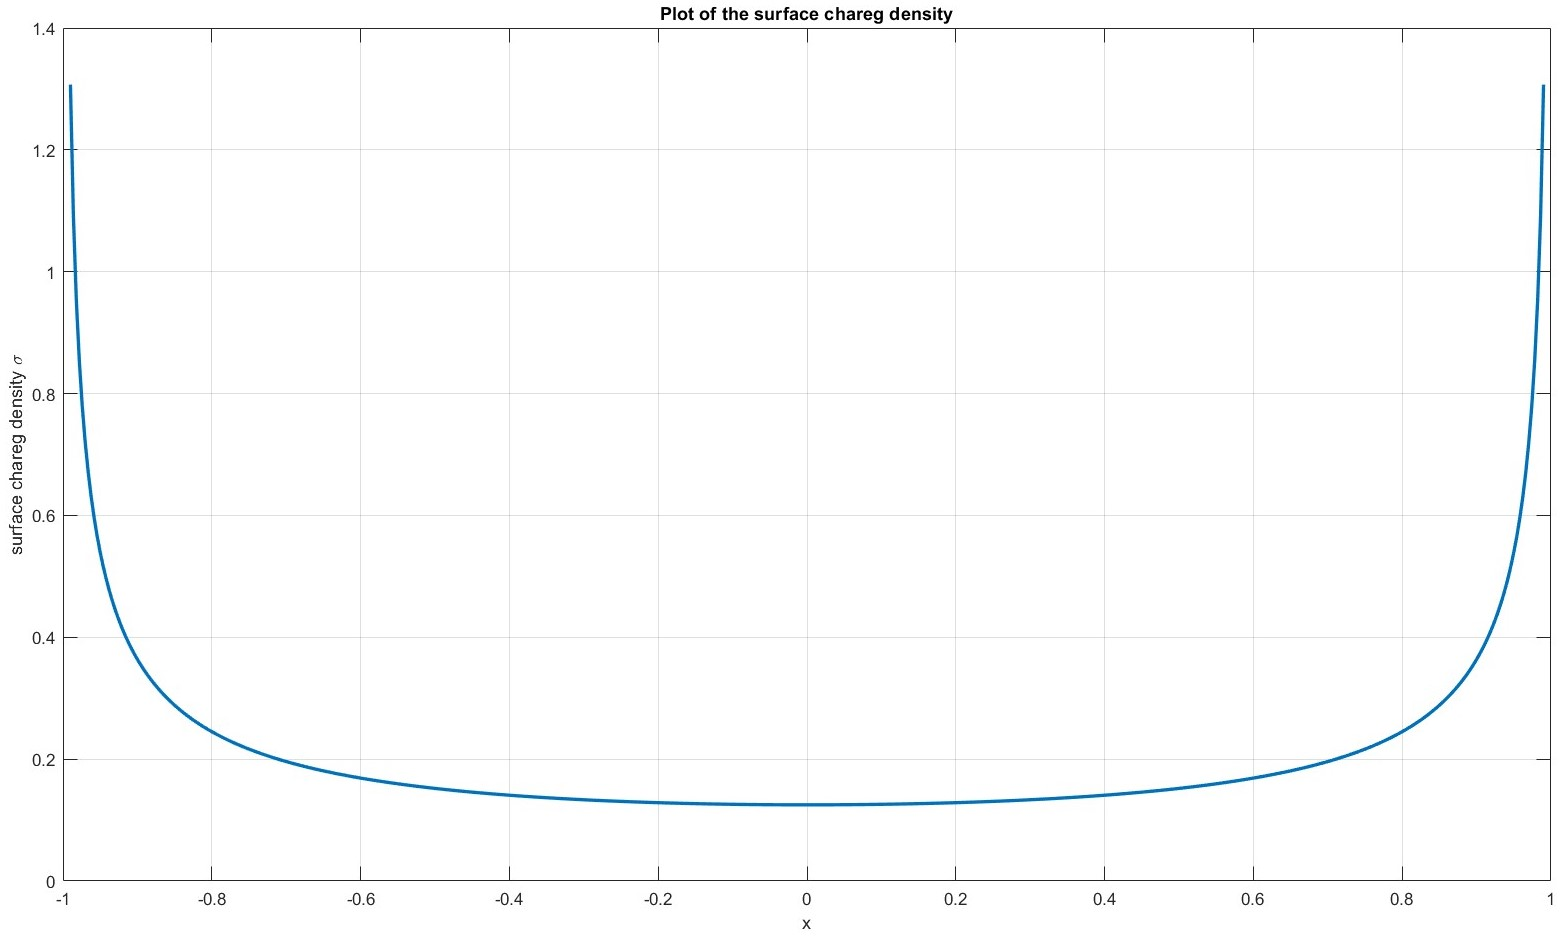
\includegraphics[width=1.\linewidth]{Figs/surface charge density.jpg}
    \caption{\small The Surface Charge Density, $x\in(-0.99, 0.99)$. At the boundary area, the value goes to $\infty$, hence omitted.}
    \label{fig:charge_d}
\end{figure}
The curve in Figure (\ref{fig:charge_d}), which represents the surface charge distribution along the droplet's upper boundary, is similar to those in \citet{Crowdy2015}, FIG. 10 of \citet{Fontelos2008}, and FIG. 2(b) of \citet{Leong2014}.

We next derive the droplet curve\footnote{\[
\int \sigma \sim \arctan \sqrt{1-x^2}
\]
}. Due to the difficulty of direct integration, we will use the Taylor expansion of $\sigma^2$:

\[\sigma^2=\frac{4}{1-x^2}\frac{1}{\left(1 + a^2 + 2 a \sqrt{1 - x^2}\right)^2}\]
Taylor expansion at $x=0$, to the second order, gives:\footnote{We attempted direct integration using numerical methods and then performed expansions at \(x = 0\), \(x = 1/2\), and \(x = 1\) respectively. From the observed results, the expansion at \(x = 0\) is the closest to the result of numerical integration. Therefore, we proceed with the derivation following the expansion at \(x = 0\) in this section.}
\[
\sigma^2\sim q^2 \left(C_1 + C_2 x^2\right)+ O(x^3)
\]
plug $\sigma^2$ into the height function:
\[
h_{xx}=\Delta p -\frac{1}{2}\sigma^2\sim \Delta p -q^2 \left(C_1 + C_2 x^2\right)
\]
integrate once find:
\[
h_x\sim \Delta p x -q^2 \left(C_1 x+ C_2 \frac{x^3}{3}\right)+D
\]
integrate twice find:
\[
h\sim \Delta p =\frac{x^2}{2} -q^2 \left(C_1 \frac{x^2}{2}+ C_2 \frac{x^4}{12}\right)+D x + C_3
\]
Based on the result above, we will use a general function for the height, incorporating some constants, where $q^2$ is included:\vspace{-1.1em}
\[
h\simeq -A x^4 + B x^2 +C x + D
\]
Apply the boundary conditions:
\begin{itemize}
    \item By the symmetry about the $y$-axis and continuity of droplet curve: \vspace{-1em}
    \[h'(0)=0\Longrightarrow C=0\vspace{-1.5em}
    \]
    \item To reduce the number of constants, we fix the height at $x=0$. \vspace{-1em}
    \[
    h(0)\coloneqq 1\Longrightarrow D \coloneqq 1\vspace{-1.5em}
    \]
    \item The slit lies on $x\in(-1, 1)$, then\vspace{-1em}
    \[
h(1)\coloneqq 0\Longrightarrow -A+B+1=0\Longrightarrow A=B+1\vspace{-1.5em}
    \]
    \item the slit is always above $y=0$\vspace{-1em}
    \[
    h(x)\geq 0\vspace{-1.5em}
    \]
\end{itemize}
hence we find
\[
h=-(B+1)x^4+B x^2+1
\]
Further investigation requires specific parameters that conform to the physical characteristics. Here, we attempt to obtain the droplet curve function with some estimated values.
\begin{figure}[H]
    \centering
    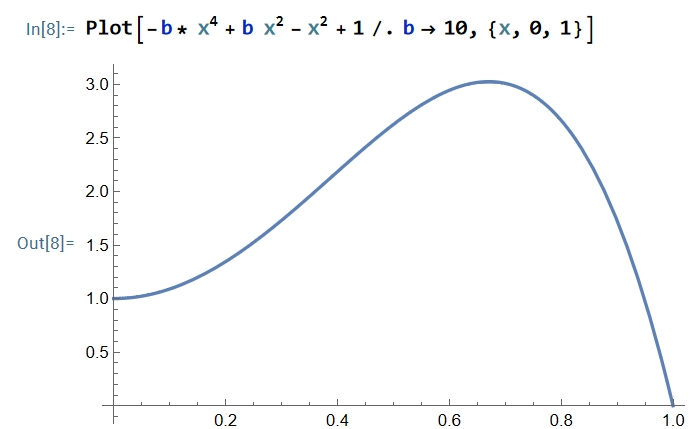
\includegraphics[width=1.\linewidth]{Figs/2d curve with q.png}
    \caption{\small The estimated curve of the droplet boundary. The $y$-axis represents the height, and the boundary $h(0)$ is fixed.}
    \label{fig:enter-label}
\end{figure}
Next, we plot the droplet curve of a varying charge magnitude $q$:
\begin{figure}[H]
    \centering
    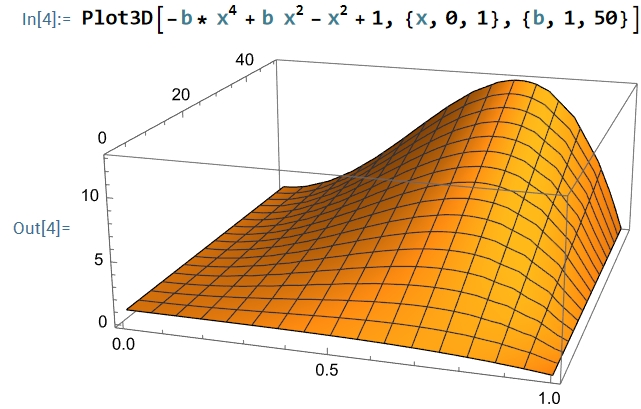
\includegraphics[width=1.\linewidth]{Figs/curve with q.png}
    \caption{\small The estimated droplet curve of the droplet boundary, with $q$ varying. The boundary $h(0)$ is fixed.}
    \label{fig:enter-label}
\end{figure}
\noindent In these plots, we observe the rise of the peak at the ends as $q$ increases, which is consistent with the research results of FIG. 2(a) \citet{Leong2014}, and FIG. 2.1. \citet{Fontelos2008_2}.